%%% ---------------
%%% PREAMBLE
%%% ---------------
\documentclass[french,11pt]{article}

% Define geometry (without using the geometry package)
\usepackage[a4paper]{geometry}
\geometry{landscape, twocolumn, textwidth=28.0cm, textheight=19.5cm, columnsep=12mm}

%\frenchspacing						% better looking spacing

% Call packages we'll need
\usepackage{graphicx}				% images
\usepackage{multicol}
\usepackage{multirow}
\usepackage{url}					% clickable links
\usepackage{marvosym}				% symbols
\usepackage{wrapfig}				% wrapping text around figures
\usepackage{fontspec}			% font encoding
\usepackage{xunicode}
\usepackage{phonenumbers}
\usepackage[hidelinks]{hyperref}
\usepackage{ragged2e}
\usepackage{pst-barcode}
\usepackage{titlesec}
\usepackage{framed}
%\usepackage[default]{raleway}
\usepackage{tocvsec2}
% Customize (header and) footer
\usepackage{fancyhdr}
\usepackage{enumitem}
\usepackage{fontawesome}
\usepackage{lipsum}
\usepackage{babel}
%\usepackage{currency}
%\pagestyle{fancy}
\pagestyle{empty}
\setmainfont{Carlito}

%\newfontfamily\headingfont[]{Arial}
%\titleformat*{\section}{\Large\bfseries\sffamily}
%\titleformat*{\section}{\Large\headingfont}

%\renewcommand{\headrulewidth}{0.0pt}	% no bar on top of page
%\renewcommand{\footrulewidth}{0.4pt}	% bar on bottom of page

%%% ---------------
%%% DEFINITIONS
%%% ---------------

% Define separators

% Define Title en News input
\newcommand{\JournalName}[1]{%
		\begin{center}
			%\Huge \usefont{T1}{augie}{m}{n}
            \Large \usefont{T1}{augie}{m}{n}
			#1%
		\end{center}
		\par \normalsize \normalfont}

\newcommand*{\chants}{../chants}
\newcommand*{\messe}{../messe_du_peuple_de_dieu}
\newcommand*{\pu}{../pu}
\newcommand*{\psaumes}{../psaumes}
\newcommand*{\footer}{..}

%\DefineCurrency{EUR}{name={euro}, plural={euros}, symbol={\euro}, iso={EUR}, kind=iso}

\newcommand{\NewsItem}[1]{%
\vspace{3pt}
\underline{\textbf{#1}}
	%	%\usefont{T1}{augie}{m}{n}
	%	\large \textbf{#1} %\vspace{3pt}
   %     %\Large #1 \vspace{4pt}
	%	%\par
   %     \normalsize \normalfont
		  }

\newcommand{\NewsAuthor}[1]{%
			\hfill by \textsc{#1} \vspace{4pt}
			\par \normalfont}
%\sisetup{locale=FR}
%\sisetup{group-minimum-digits=3}

\graphicspath{{../images/}}

%pas de numérotation des sections
\setsecnumdepth{none}
\setlength{\parindent}{0pt}
%%% ---------------
%%% BEGIN DOCUMENT
%%% ---------------
\begin{document}

\NewsItem{CHANT D'ENTRÉE}\\
	\textbf{
Chantez, priez, célébrez le seigneur,
Dieu nous accueille, peuples du monde.\\
Chantez, priez, célébrez son nom,
Dieu nous accueille dans sa maison.
}

\begin{tabular}{p{0.5\columnwidth} p{0.5\columnwidth}}
1.
Il a fait le ciel et la terre,\newline
ÉTERNEL EST SON AMOUR,\newline
Façonné l’homme à son image,\newline
ÉTERNEL EST SON AMOUR.
&
%2
%Il sauva Noé du déluge,
%ÉTERNEL EST SON AMOUR,
%L’arc-en-ciel en signe d’alliance,
%ÉTERNEL EST SON AMOUR.
%
%3
%D’Abraham, il fit un grand peuple,
%ÉTERNEL EST SON AMOUR,
%Par milliers fut sa descendance,
%ÉTERNEL EST SON AMOUR.
%
%4
%Il perçut le cri de son peuple,
%ÉTERNEL EST SON AMOUR,
%Le guida en terre promise,
%ÉTERNEL EST SON AMOUR.
%
%5
%Aux exilés de Babylone,
%ÉTERNEL EST SON AMOUR,
%Il donna la foi qui libère,
%ÉTERNEL EST SON AMOUR.

6.
Il a parlé par les prophètes,\newline
ÉTERNEL EST SON AMOUR,\newline
Sa parole est une promesse,\newline
ÉTERNEL EST SON AMOUR.
\end{tabular}


\NewsItem{PRÉPARATION PÉNITENTIELLE}\\
	Seigneur, prends pitié. Seigneur prends pitié, Seigneur, prends pitié\\
Ô Christ, prends pitié. ô Christ prends pitié, o Christ, prends pitié.\\
Seigneur, prends pitié. Seigneur, prends pitié Seigneur, prends pitié


\NewsItem{GLORIA}\\
	\begin{itemize}
\item[R/] 
Gloire à Dieu, au plus haut des cieux, et paix sur la terre, aux hommes qu'il aime. (bis)
\item[1.]
Nous te louons, nous te bénissons, nous t’adorons, nous te glorifions, nous   
      te rendons grâce pour ton immense gloire. Seigneur Dieu, Roi du ciel, Dieu 
      le Père tout puissant. R/
\item[2.]
Jésus-Christ, Seigneur Fils unique, Agneau de Dieu, le Fils du Père, toi qui 
      enlèves le péché du monde, reçois nos prières. Toi qui es assis à la droite  
      du Père, prends pitié de nous. R/
\item[3.]
Car toi seul es saint, toi seul es Seigneur, toi seul es le Très Haut : 
      Jésus-Christ, avec le Saint Esprit, dans la gloire de Dieu le Père. R/
\end{itemize}




% -----
\NewsItem{1\iere{} LECTURE} Ex 17, 8-13
% -----

\NewsItem{PSAUME}
Ps 120 (121), 1-2, 3-4, 5-6, 7-8

\textbf{Le secours me viendra du Seigneur
qui a fait le ciel et la terre.}

Je lève les yeux vers les montagnes :
d’où le secours me viendra-t-il ?
Le secours me viendra du Seigneur
qui a fait le ciel et la terre.

%\smallskip

Qu’il empêche ton pied de glisser,
qu’il ne dorme pas, ton gardien.
Non, il ne dort pas, ne sommeille pas,
le gardien d’Israël.

%\smallskip

Le Seigneur, ton gardien, le Seigneur, ton ombrage,
se tient près de toi.
Le soleil, pendant le jour, ne pourra te frapper,
ni la lune, durant la nuit.

%\smallskip

Le Seigneur te gardera de tout mal,
il gardera ta vie.
Le Seigneur te gardera, au départ et au retour,
maintenant, à jamais.


% -----
\NewsItem{2\ieme{} LECTURE} 2 Tm 3, 14 – 4, 2

\NewsItem{ACCLAMATION}
Alleluia \emph{messe du Peuple de Dieu}


\NewsItem{ÉVANGILE} Lc 18, 1-8

\NewsItem{HOMÉLIE}

\NewsItem{PROFESSION DE FOI}
%\textbf{Je crois en Toi Père, Fils et Esprit. J’ai confiance en Toi, Tu es mon ami.}


\begin{tabular}{p{0.5\columnwidth} p{0.5\columnwidth}}
1 - Père Créateur de vie, nous sommes tes enfants, Tu nous donnes la vie, 
  Toi qui nous aimes tant.
&
2 - Jésus né de Marie, Tu es le Fils de Dieu. Tu nous 
  donnes Ta vie comme un cadeau précieux.
\\
3 - Et Toi Esprit de Dieu, Tu nous 
  donnes Ta force, un souffle silencieux nous unit, nous renforce.
&
4 - Je crois 
 que je grandis en Te confiant ma vie, ma famille, mes amis, au nom du Père, 
  du Fils et de l’Esprit.\newline
  Amen. Amen. Amen. 
\end{tabular}




%\newpage

\NewsItem{PRIÈRES UNIVERSELLES}
Accueille au creux de tes mains la prière de tes enfants.

%Par ta Sainte Mère Seigneur nous te prions


\NewsItem{OFFERTOIRE}

\NewsItem{PRIÈRES SUR LES OFFRANDES}\\
\textit{Nous nous levons et nous répondons : }
Que le Seigneur reçoive de vos mains ce sacrifice à la louange et à la gloire
de Son nom, pour notre bien et celui de toute l’Église.


\NewsItem{SANCTUS}
Le Seigneur est Saint ! Le Seigneur est Saint ! Le Seigneur est Saint !
Le Seigneur est notre Dieu, Le Seigneur est notre Père. Il règne dans les cieux, qu’Il règne sur la terre.


\NewsItem{ANAMNÈSE}
Christ est venu, Christ est né, Christ a souffert, Christ est mort, 
Christ est ressuscité, Christ est vivant,
Christ reviendra, Christ est là,
Christ reviendra, Christ est là.


\NewsItem{NOTRE PÈRE}

\NewsItem{AGNUS} \\
Agneau de Dieu Qui enlèves le péché du monde, Prends pitié de nous !  Prends pitié de nous ! (bis) \\
Agneau de Dieu Qui enlèves le péché du monde, Donne-nous la paix !  Donne-nous la paix !


\NewsItem{COMMUNION} \textbf{orgue}
%\NewsItem{COMMUNION} \textbf{orgue} ou
%\\
\textbf{Fais nous entrer en communion avec toi et tous nos frères.}


\begin{tabular}{p{0.5\columnwidth} p{0.5\columnwidth}}
 1. Seigneur, tu nous invites à la table \newline
 Où tu nous partages ta Parole,\newline
 Le Pain rompu pour notre vie.
&
 2. Seigneur, tu nous invites à l’écoute,\newline
 À manger et boire ta Sagesse,\newline
 Festin des noces de la vie. 
\\
3. Seigneur, tu nous invites à la Cène \newline
Où tu nous saisis dans ton Alliance\newline
Parole et Pain de notre vie. 
&
4. Seigneur, tu nous invites à l'audace\newline
De ceux qui te donnent leur confiance\newline
En te laissant saisir leur vie.
\end{tabular}


\NewsItem{ANNONCES PAROISSIALES}


\NewsItem{CHANT D'ENVOI}
%Mystères joyeux

\textbf{
Réjouis-toi, Marie,
Mère du Christ et notre Mère !
Dieu t’a donné son Fils
Pour le bonheur de notre terre.
}

\begin{tabular}{@{}p{0.5\columnwidth} p{0.5\columnwidth}@{}}
1.
L’ange de Dieu t’a saluée,\newline
Pleine de grâce, ô Marie !\newline
En toi le Verbe s’est fait chair,\newline
Bénie sois-tu pour ton oui !
&
2.
Tu fais la joie d’Elisabeth\newline
Par ta visite, ô Marie !\newline
De toi jaillit magnificat,\newline
Le chant nouveau dans l’Esprit.
\end{tabular}


\newpage

%\NewsItem{Intentions de messe}
%\begin{itemize}
%\item[\Cross] Françoise et André BOUCHEZ et les défunts de la famille (Sainte Croix)
%\end{itemize}

\NewsItem{Informations paroissiales}

\begin{tabular} {lcp{9cm}}
\multicolumn{3}{c}{\textbf{Saint Jean-Baptiste} } \\ \hline
Mardi    & 21 oct.  & Vêpres 18h15. Messe 18h30 \\ \hline
Jeudi    & 23 oct. &
Exposition du Saint Sacrement à 16h00. Adoration. Salut au Saint Sacrement à 18h15. Messe à 18h30 
 \\ \hline
Vendredi & 24 oct. & Laudes 08h45. Messe 09h00 \\ \hline
Samedi   & 25 oct. & Messe anticipée 18h00 \\ \hline
Dimanche  & 26 oct. & Messe 11h00\\ \hline
\multicolumn{3}{c}{\textbf{Sainte Croix} } \\ \hline
Mercredi & 22 oct.  & Messe 09h00. \\ \hline
%\newline \Cross{} \textbf{Enterrement}  14h30 Marie-Claire Noël \\ \hline
%Dimanche  & 26 oct. & \textbf{messe unique} 10h00\\ \hline
Dimanche  & 26 oct. & Messe 09h30\\ \hline
%\multicolumn{3}{c}{\textbf{Résidence Landsberg (3 rue Jean Monnet)} } \\ \hline
%Mercredi & 01 oct. : & Messe 10h45 \\ \hline
\end{tabular}

\begin{framed}
\begin{itemize}
\item
Semaine missionaire mondiale. Du 12 au 19 oct.
\item
Pour les collégiens et lycéens : \textbf{Apéritif de rentrée du groupe des jeunes} ven. 24 oct. 18h00 au presbytère. QR code WhatsApp au fond de l'église.
\item Ven. 14 nov. 19h00 : \textbf{repas harengs} au foyer Ste Croix. Réservation avant le 07 novembre au \phonenumber[country=FR]{0683825250} ou \texttt{foyer.sainte.croix@gmail.com}
\item
Concert \textbf{Glorious} dim. 14 déc. au Zénith de Strasbourg à 18h00. 35~€ par personne. La paroisse prend en charge 10~€ pour les collégiens et lycéens. Contact Nathalie ou Louise \texttt{nathalie\_dick@yahoo.fr} jusqu'au 31 oct.
\item
\textbf{Confessions} au presbytère : les 1\iers{} jeudis du mois de 16h à 17h30. Les 3\iemes{} samedis du mois de 15h à 16h30.
\end{itemize}
\end{framed}

\NewsItem{Répétitions des chorales}
\begin{description}
\item[Chorales paroissiales] : vendredi 20h15 à Sainte Croix
\end{description}

\begin{framed}
\textbf{Presbytère St Jean-Baptiste}
%2 rue de l'école 67380 Lingolsheim 03 88 78 16 45 \\
2 rue de l'école 67380 Lingolsheim \phonenumber[country=FR]{0388781645} \\
\textbf{Permanence} Lun. au Jeu. : 09h30-12h00 et 15h-18h. Ven. 16h-18h00. Sam. 09h30-12h00. \\
\textbf{Courriels} \texttt{nddessables@hotmail.com}, \texttt{danielette67380@gmail.com}

%\textbf{Caritas} Vestiaire ouvert le mardi de 14h à 16h

\texttt{https://stjeanbaptistelingo.fr} \hfill \faFacebook Catho Lingo \hfill \faInstagram @catho\_lingo
\end{framed}



\newpage

\JournalName{Communauté de Paroisses de Lingolsheim \\
\normalsize \textit{Notre Dame des Sables}
%\\ \large \'{E}glise Saint Jean-Baptiste
\\  \normalsize \textit{29\ieme{} dimanche du Temps Ordinaire - C}
\\ \large Samedi 18 octobre 2025}
%\noindent\HorRule{3pt} \\[-0.75\baselineskip]
%\HorRule{1pt}
% -----

% Front article
% -----
%\vspace{0.5cm}
%	\SepRule
%\vspace{0.5cm}

%\begin{center}
\begin{minipage}[h]{1.0\linewidth}
\setlength{\parindent}{1em}
 \begin{center}
 \textbf{
 %\dots
\og 
Rentrée Pastorale 2025-2026
 \fg{}
 %\dots
 }
 \end{center}

%\begin{wrapfigure}{l}{1.3cm}
%\vspace{-0.4cm}
%	\includegraphics[scale=1.0]{../images/lazarre}
%\end{wrapfigure}
Une nouvelle rentrée pastorale qui nous réjouit tous. En effet, après un temps de répit, il nous revient de mettre en marche la machine de nos activités pastorales.

Au début de cette nouvelle année pastorale, je souhaite vous redire toute ma joie de vous retrouver pour continuer la mission qui m’est assignée dans notre communauté de paroisses. Et comme chaque année, nous mettrons l’accent en premier lieu sur la vie catéchétique des enfants et des adolescences, l’animation liturgique, la création d’une troisième chorale, la visite aux malades et dans notre maison de retraite ( \emph{Résidence du Parc}), l’accueil et l’accompagnement en vue de baptêmes,  du catéchuménat des adultes, des mariages, l’encadrement  des servants d’autel, l’entretien de notre église pour la rendre  accueillante, avec ces innombrables petits gestes de service qui jalonnent l’existence ; tout cela nous aidera à vivre une véritable dimension ecclésiale.

Je voudrais vous remercier de tout cœur, vous tous qui êtes des membres vivants et actifs de la communauté paroissiale que nous formons, véritable artisans de l’évangélisation ordinaire. Mon souhait pour la vie de notre communauté de paroisses est que nous arrivions toujours plus à nous ouvrir et à nous connaître les uns les autres, à nous apprécier dans ce que nous sommes et vivons.

L’année dernière, avec toutes les entités de nos deux paroisses, nous avons eu différentes propositions, activités et invitations qui ont favorisées l’\textbf{Unité et l’ouverture} qui constituaient notre thème pastoral. Ne manquons pas cette année ces moments simples et conviviaux qui permettent de tisser des liens gratuits, profonds et tout simplement chrétiens.

\begin{wrapfigure}{l}{1.2cm}
\vspace{-0.4cm}
	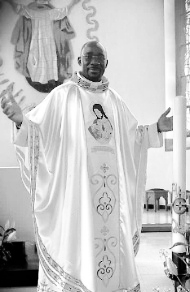
\includegraphics[scale=1.20]{../images/standing_daniel}
\end{wrapfigure}
Cette année nous porterons ensemble cette rentrée dans le cœur de chacun avec nos \textbf{jeunes pro}. Chacun à son rythme, selon ses possibilités et ses réalités mais avec un seul et même objectif : l’accomplissement de nos activités communautaires. Présentons également notre rentrée paroissiale au Christ. Et continuons notre chemin pour la mise en œuvre de notre projet paroissial autour de ce principal thème : \textbf{\og Avec notre jeunesse bâtissons une communauté plus dynamique, rayonnante et missionnaire\fg{}.}

	Que cette rentrée pastorale nous aide à prendre des résolutions nécessairement pour plonger à frais nouveaux dans la parole et être des disciples crédibles de l’évangile.


\begin{flushright}
Bonne rentrée pastorale à toutes et à tous !
\textit{Père  Daniel  ETTÉ}
\end{flushright}


\end{minipage}
%\end{center}
% -----
\end{document}
